\documentclass[titlepage]{article}
\usepackage[T1]{fontenc}
\usepackage[utf8x]{inputenc}
\usepackage{placeins}
\usepackage{graphicx}
\usepackage[english]{babel}


\author{Luca Massini \and Daniele Nicolò}

\title{Design Document
\\  Safestreets}

\date{release date to be defined}
\begin{document}
\maketitle
\newpage 
\tableofcontents
\newpage
\section{Introduction}
\subsection{Purpose}
	This document is necessary to describe the architecture of the system from several points of view. This document has the scope of giving more details (especially to developers) about the system to be in terms of system architecture, in terms of software implementation and in terms of integration and testing. This document follows a top down approach. In fact as the reader will proceed toward the end of the document there will be an increasingly detailed description of all the design aspect concerning the system.
\subsection{Scope}
Safestreets is a service that allows private users to inform authorities about parking and traffic violations. A user must take a picture of the violation and describe it and the place where it occurred. An image recognition algorithm is run on the sent picture. A user has also the possibility to see the safety of the streets and the parking areas and to check the most reported streets and vehicles. \\
The system offers also the possibility to receive suggestions in order to improve the streets safety. This feature is available only for municipality accounts. These  suggestions are generated by the system using an algorithm that retrieves the information from the users' reports and also from the data given by the municipality.
\subsection{Definitions,Acronyms and Abbreviations}
\subsubsection{Definitions}
TODO
\subsubsection{Acronyms}
TODO
\subsubsection{Abbreviations}
TODO
\subsection{Revision History}
TODO
\subsection{Reference Documents}
TODO
\subsection{Document Structure}
The following sections are structured as below:
\begin{itemize}
	\item \textbf{Architectural Design: }In this section there will be the description of the system from the architectural point of view. This means to show the components and their interactions with each other and to explain the design patterns choices and the architectural styles. 
	\item \textbf{User Interface Design:} In this section there is an explanation,in terms of user experience (UX), of the user interfaces already showed in the RASD mockups.
	\item \textbf{Requirements Traceability:} Here we describe how the requirements already explained in the RASD match with the design choices done in this document.
	\item \textbf{Implementation, Integration and Test plan:} Here there is the description of how we will implement all the components, how we will integrate them together and finally how we will test both the single components and also the integrated system.
	\item \textbf{Effort spent:} Here there is the division of the work hours of each member of the group and the description of the tasks completed and related time spent.
\end{itemize}
\begin{figure}[h]
\section{Architectural Design}
	\subsection{Overview}
In the figure below it is shown the architecture of the entire system. This description has to be intended only as an overview and because of this some details are not shown.
	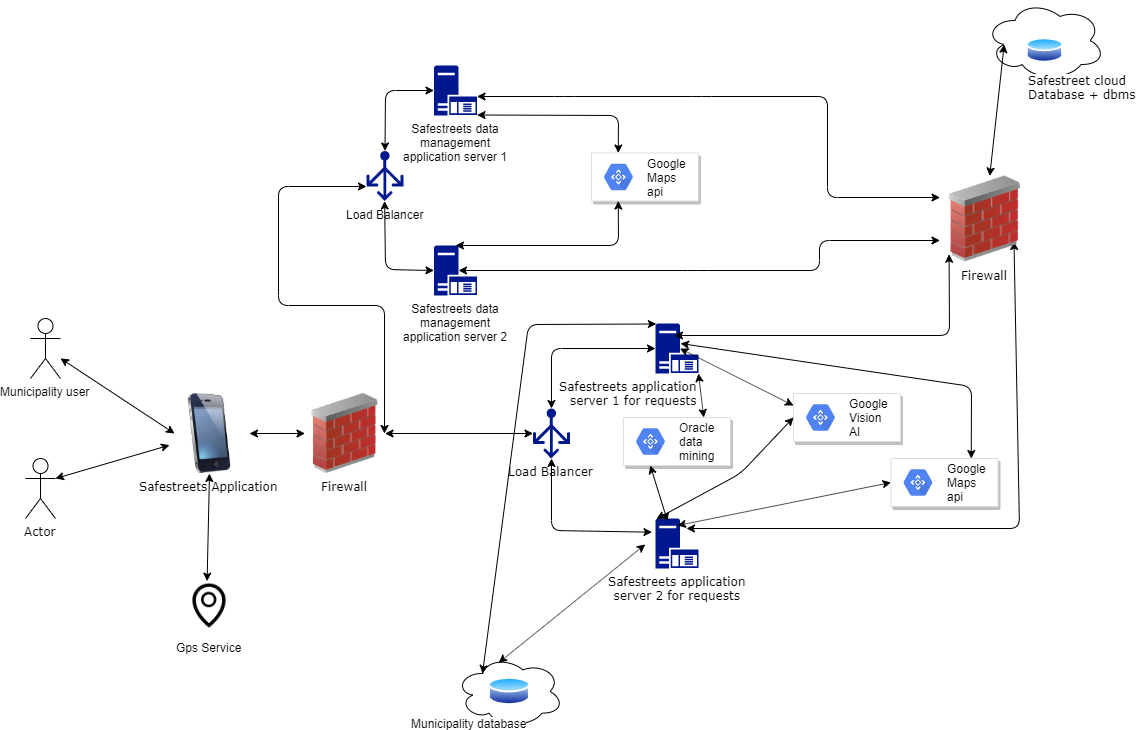
\includegraphics[scale=0.465]{Diagrams/overview.png}
	\caption{Architectural overview}
\end{figure}
\FloatBarrier

In this overview we can immediately distinguish the architectural layers. Servers manage the logic one whereas databases manage the data layer and finally the client smartphone is where the presentation layer resides. \\
The architecture has 2 clusters. Every server contained in one cluster access the system database whereas instead only the two databases dedicated to requests access the external one (which is the external database of the municipality). Servers which resides in different clusters don't communicate with each other to guarantee the service. Also servers of the same cluster don't communicate with each other obviously. The workload balancing between servers of the same cluster will have to work thanks to load balancers.\\
The client in order to receive the service will speak directly and only to the firewall placed at the entrance of the system. The first firewall (the one near the SafeStreets application in the diagram) is the element that will rout the user message to the right cluster based on the type of request. In this case that firewall has not only a security function (obviously the main function of a firewall is that) but it also behaves as a gateway which routes packets. All the clusters are placed inside the DMZ (between two firewalls) for security reasons. They must be accessible from outside the internal network. The second firewall divides clusters from the system database. The database will have to be accessible only from the clusters for security reasons and because of this fact they are outside of the DMZ.\\
The fact that we have two independent servers per cluster that offers the same services will cost more for sure but we want this system to be discreetly fault-tolerant and performing. A solution with only one server would have been too much dangerous in the terms expressed just above.
\subsection{Component view}
Here there is a description of the software components that will be implemented in the specific hardware.

\begin{figure}[h]
	\includegraphics[scale=0.1]{Diagrams/Component diagram.png}
	\caption{Component diagram}
\end{figure}
\FloatBarrier

With this diagram our purpose is to show the internal software architecture of SafeStreets. \\
The main components are the user client application, the requests server application and the data management server. The external interfaces are SafeStreets cloud database, the municipality database and the GPS interface.\\
These main components contain smaller modular components that communicate with each other and with the external interfaces to complete different functions.\\
Now we will describe the internal components and the external interfaces in detail. \\

\paragraph{\textbf{User Client Application}}
The User Client Application is situated in the user's smartphone. It contains the Data Manager, the View and the Communication Manager:
\begin{itemize}
\item \textbf{Data Manager}\\
This component is responsible of taking the user's position in the world using the GPS service offered by his smartphone. Those data will be sent to the server in case he selects a service that uses the GPS localization. \\
\item \textbf{View}\\
This component is the view part of the MVC pattern. It takes data provided by the controller situated in the Server and shows them to the user with its interface.
\item \textbf{Communication Manager}\\
The Communication Manager is responsible for the network.
It manages all the communication from the client to the server and vice versa.\\
\end{itemize}




\begin{figure}[h]
	\subsection{Deployment view}
	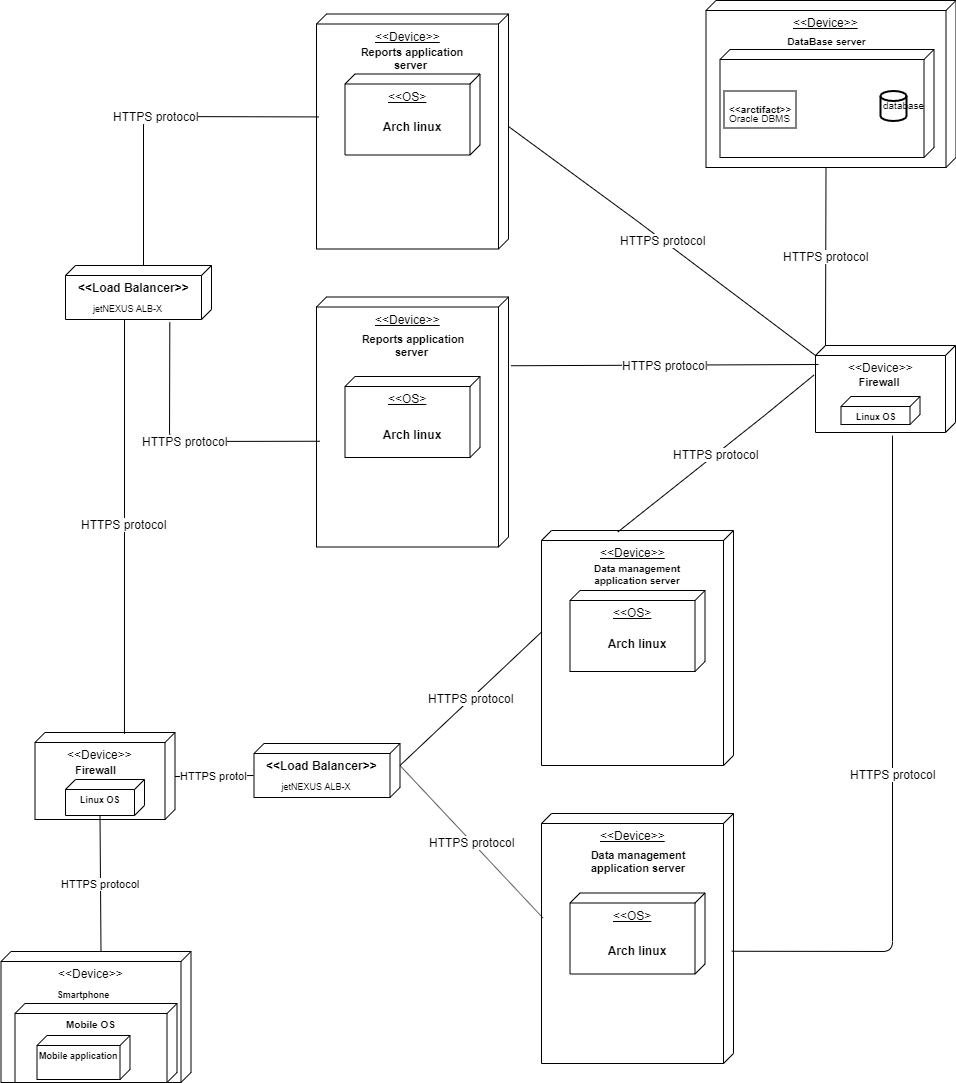
\includegraphics[scale=0.465]{Diagrams/Deployment diagram.png}
	\caption{Deployment diagram}
\end{figure}
\FloatBarrier

This diagram is very similar to the one in the overview. It express some aspects which have been already explained and some others are explained only here. In fact we can see all the operating systems for each server and also the protocol used in the communication between the devices.
Here you can find a brief description of what the single components do:
\begin{itemize}
\item \textbf{Firewall:} Firewalls are well known for sure by the majority of the people but we think that it is important to describe their operation the same. Firewalls are placed between the internal network and the external ones.They are used to filter the incoming/outcoming packet traffic. Through a set of rules they decide if a packet can pass or (unique alternative) be blocked.  This can be very useful to guarantee a better system safety.
\item \textbf{Load Balancer:} Load Balancers are used to improve the workloads across multiple computing resources. Thanks to load balancer the load can be balanced in an optimal way.This can make the system more performing and can also improve the fault tolerance of the system because of redundancy.
\item \textbf{Servers:} In this architecture we can find two clusters, each one containing 2 application servers. The servers are specialized with no overlap of functionalities. One is specialized in the managing of the reports by the private users. It must update the database with the new incoming data only after having done all the checks about the validity and correctness of the report.\\
The other server deals with the managing of the requests by the private users or municipalities. It is in charge of check the correctness and validity of the request,and then it must run all the data mining algorithms necessary to retrieve the result and finally send the results to the right private user.
\item \textbf{Databases:} The databases are cloud databases managed thanks to an API that will be provided by the provider of the service. We have only one cloud database used to store all the Safestreets data. Another cloud database is the external one of the municipality. Safestreets has only a special view of the part of the municipality database concerning the accidents. All these cloud database use SQL.
\end{itemize}
\subsection{Runtime View}
\subsection{Component interfaces}
\subsection{Selected architectural styles and patterns}
We have selected an 4 tiers architecture. The entire system is a client-server application. The smartphone of the user has only the presentation layer which changes when the client send a request to the server (that can be a request or a report). This decision is due to the fact that we want the mobile application to be lightweight. We want the app to perform discreetly even with non-modern hardware phones. We want an application that limits as little as possible the hardware in a phone in terms of performance. The system data are stored in a database  whereas the systems uses also another database which is the one of the municipality.
The application logic is divided in two specialized clusters of application servers as already explained. We have chosen this to make the two interactions with the user (a user request or a user report) independent as much as possible.\\
 The data layer is implemented in the databases of the system.\\
The decision of having different layers is to make the system as maintainable as possible. Every layer will offer only a simple interface to receive data and another one to send data to another layer and nothing more. In this way the implementation details are hidden. This means that when the system is modified it cannot happen that the modification of a layer causes a chain of successive modifications in other layers caused by the latter.\\ \\
The system can be seen as an example of MVC pattern:
\begin{itemize}
	 \item \textbf{Model:} The model is the component which store all the application data and check their integrity and so eventually modify the data structures to keep it. It is implemented in the databases (both the external and the internal one)
	 \item \textbf{View:} The view is the software component that deals with the presentation layer. It only show data and information to the user. This component is implemented in the user device (as already explained before)
	 \item \textbf{Controller:} The controller is the software component that contains and manages the application logic. In this system this logic layer must be implemented in the application servers. \\
In our case, in particular, it is divided in two subcomponents. One part concerns the managing of the requests and the other one concerns with the reports of the user. The first its implemented in the servers for the request and the latter in the servers for the reports.
\end{itemize}
\subsection{Other design decisions}
Here it is possible to find another design decision which are not about patterns and design styles which are the following:
\begin{itemize}
	\item \textbf{ Use of cloud databases:} We have chosen cloud databases to store the systems data because in this way it is possible to decrease or increase the resources according to the load of requests or reports. In this way it is possible to balance the storage space according to the load automatically. A solution based on proprietary databases would have been probably more efficient in terms of performances but surely more critical in terms of allocation or deallocation of resources. Furthermore, another important aspect of this choice is the fact that the physical maintenance of cloud database is entrusted to third parties (the owners of the physical devices which are the providers of the cloud service).
	\item \textbf{Use of clusters:} The use of clusters has been decide in order to try to make the system possibly more performing but above all, more fault tolerate. We have discarded the idea of having a single server instead of a cluster precisely because of this aspect. If the single server is down, then, the entire service will surely be inaccessible for the user. \\
The use of clusters is excellent as it makes the system more scalable. In fact, it is also easy to add additional servers.
	\item \textbf{Use of load balancers:} The use of load balancers has been decided to make the system more performing. In fact the throughput can be maximized and the response time minimized as much as possible. 
	\item \textbf{Use of relational databases:} For this system we have chosen relational databases. On of the reason about this decision is the fact that the data that the system manages and stores is well defined and structured. We know that sometimes operations like "join" between different tables can affect the system and make it slower. However, we think that this aspect will not cause relevant problems in our system. In fact the performance constraints are large enough to not cause problems in our opinion. Furthermore, relational databases have been used for several years and they are used also nowadays for a lot of applications. Because of this, we have a strong theoretical background about them.
	
\end{itemize}

\begin{figure}[h]
	\section{User interface design}
Here there will be shown the user interfaces with the help of UX diagrams. In particular there is shown the flow that the user will follow to navigate inside the application. Some aspects concerning the user interfaces design have been already treated in the "Requirement Analysis and Specification Document",if the reader wants to understand in a better and more detailed way, he/she is strongly suggested to refer also to it. In this document it is described only the flow that the user must follow to use the application.
UX diagrams:\\
	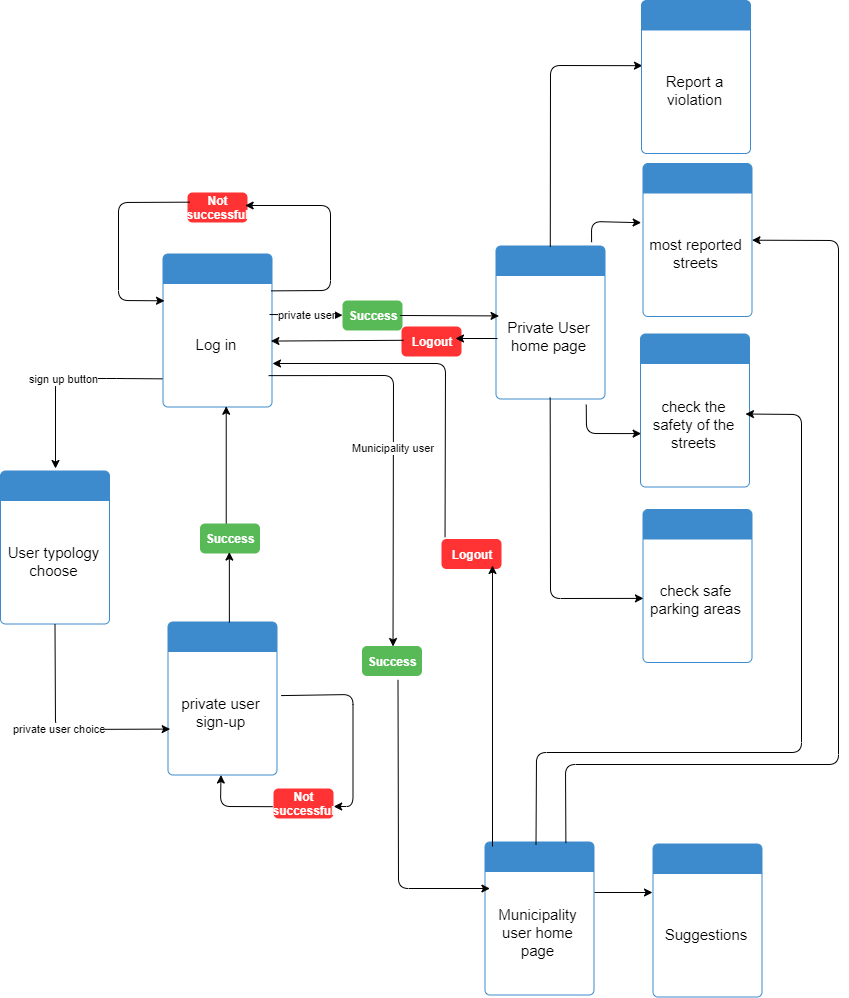
\includegraphics[scale=0.48]{Diagrams/UX diagram.png}
	\caption{UX diagram}
\end{figure}
\FloatBarrier

\section{ Requirements Traceability}

\end{document}